\chapter{Bausteinsicht}

Um ein besseres Verständnis über die Struktur des Systems zu bekommen, nutzen wir die Bausteinsicht. Sie hilft dabei ein gemeinsames Verständnis des Systems innerhalb des Teams zu bekommen.
Die zur Zerlegung benutzte Dekompistionsstrategie ist funktional. 

\section{Bausteinsicht Level 1}
 

\begin{figure}[h] % [h] = here
    \centering
    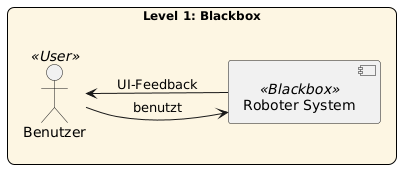
\includegraphics[width=0.6\textwidth]{diagrams/bausteinsicht_lvl_1_v2.png}
    \caption{Bausteinsicht Level 1}
\end{figure}

\begin{table}[h!]
\centering
\begin{tabular}{|p{4cm}|p{9cm}|}
\hline
\textbf{Komponente} & \textbf{Beschreibung} \\ \hline
Roboter System & Gesamtsystem, das alle internen Steuer-, Safety- und Kommunikations­funktionen kapselt. Empfängt Bedien-/Steuerbefehle vom Benutzer, verarbeitet sie und liefert Feedback. \\ \hline
\end{tabular}
\caption{Bausteinsicht Level 1 Komponenten}
\label{tab:lvl1}
\end{table}

\newpage

\begin{figure}[h] % [h] = here
    \centering
    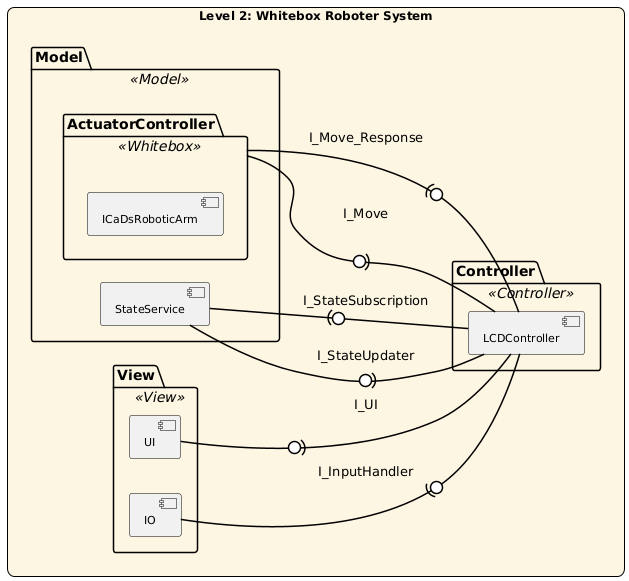
\includegraphics[width=0.6\textwidth]{diagrams/bausteinsicht_lvl_2_v2.png}
    \caption{Bausteinsicht Level 2}
\end{figure}

\begin{table}[htbp]
\centering
\begin{tabular}{|l|l|p{8cm}|}
\hline
\textbf{Komponente} & \textbf{Paket} & \textbf{Beschreibung} \\
\hline
\texttt{UI} & View & Die Benutzeroberfläche zur Darstellung von Informationen für den Nutzer. \\
\hline
\texttt{IO} & View & Eingabekomponene für den Nutzer. \\
\hline
\texttt{LCDController} & Controller & Steuert den Informationsfluss zwischen UI, IO und den Modulen des Models. \\
\hline
\texttt{StateService} & Model & Verantwortlich für die Verwaltung und Aktualisierung des internen Systemzustands. \\
\hline
\texttt{ActuatorController} & Model & Steuerlogik für Aktoren des Roboters; enthält ICaDsRoboticArm. \\
\hline
\texttt{ICaDsRoboticArm} & ActuatorController (Model) & Konkreter Baustein zur Ansteuerung eines robotischen Arms. \\
\hline
\end{tabular}
\caption{Bausteinsicht Level 2 Komponenten}
\label{tab:whitebox-komponenten}
\end{table}



